\documentclass[a4paper,11pt]{exam}
	\usepackage{graphicx}
	\usepackage[utf8]{inputenc}
	\usepackage[T1]{fontenc}
	\usepackage{listings}
	\usepackage{color}
	\usepackage{amsmath}
	\usepackage{enumerate}
	\usepackage{caption}
	\usepackage{verbatim}
	\usepackage{subcaption}
	\usepackage{tikz}
	\usepackage{graphics}
	\usepackage{txfonts}
	\usepackage{listings}
	\definecolor{dkgreen}{rgb}{0,0.5,0}
	\definecolor{gray}{rgb}{0.5,0.5,0.5}
	\definecolor{mauve}{rgb}{0.58,0,0.82}

	\lstset{frame=tb,
	  language=Python,
	  aboveskip=3mm,
	  belowskip=3mm,
	  showstringspaces=false,
	  columns=flexible,
	  basicstyle={\small\ttfamily},
	  numbers=none,
	  numberstyle=\tiny\color{gray},
	  keywordstyle=\color{blue},
	  commentstyle=\color{dkgreen},
	  stringstyle=\color{mauve},
	  breaklines=true,
	  breakatwhitespace=true
	  tabsize=3
	  }
\begin{document}
\begingroup 
	  \bf \Large Eletromagnetismo\\
	  \indent \normalsize André Del Bianco Giuffrida
	\endgroup
	\\ \quad
	\\
	\large{
	\emph{Lista 3 \\ Ex 5}
        \\
	\\ \indent Uma carga pontual $q$ se encontra frente a uma esfera condutora de raio $R$, a uma distância $d > R$ do seu centro. A esfera se encontra a um potencial $V_0 \ne 0$.
        \\
        \\
        (a) \indent Usando o método das imagens, determine o potencial elétrico fora da esfera. 
        \\
        (b) \indent Determine a densidade de carga induzida sobre a esfera.
        \\
        (c) \indent Calcule a força entre a carga e a esfera. Verifique o comportamento limite para $d >>R$.

	\normalsize


	\begin{center}
		\begin{tikzpicture}
		  \draw (0,0) circle (1.5);
		  \draw (-2,0) -- (10,0);
                  \draw (0,0.2) -- (0,-0.2) node[below] {$0$};
                  %\draw[fill=black] (0,0) circle (0.1) node[above , shift={(0,0.2)} ] {$q_0$};
                  %\draw (0.7,0.2) -- (0.7,-0.2) node[below] {$d'$};
                  %\draw[fill=black] (0.7,0) circle (0.1) node[above , shift={(0,0.2)} ] {$q'$};
                  \draw (8,0.2) -- (8,-0.2) node[below] {$d$};
                  \draw[fill=black] (8,0) circle (0.1) node[above , shift={(0,0.2)} ] {$q$};
		\end{tikzpicture}
	\end{center}
	(a)\\
	\indent Podemos considerar a configuração asseguir como problema imagem retirado do livro de referência  (Griffiths, D. J.) "Eletrodinâmica p. xv, 3a ed Pearson Addison Wesley, 2011" nesse problema o potencial na esfera é zero, para sanar essa diferença podemos inserir a carga $q_0$ na origem, onde essa garante que o potencial na esfera seja $V_0 \ne 0$.
	
	\begin{center}
		\begin{tikzpicture}
		  \draw[dashed] (0,0) circle (1.5) node[above , shift={(1,1.2)}] {$V_0$};
		  \draw (-2,0) -- (10,0);
                  \draw (0,0.2) -- (0,-0.2) node[below] {$0$};
                  \draw[fill=black] (0,0) circle (0.1) node[above , shift={(0,0.2)} ] {$q_0$};
                  \draw (0.7,0.2) -- (0.7,-0.2) node[below] {$d'$};
                  \draw[fill=black] (0.7,0) circle (0.1) node[above ,shift={(0,0.2)}] {$q'$};
                  \draw (8,0.2) -- (8,-0.2) node[below] {$d$};
                  \draw[fill=black] (8,0) circle (0.1) node[above , shift={(0,0.2)} ] {$q$};
		\end{tikzpicture}
	\end{center}
	
	\indent Nessas condições:
		
		Para satisfazer a condição de contorno, $ q_0 = 4 \pi \epsilon_0 R V_0 $
		
	\[ V(\vec{r}) = \frac{1}{ 4 \pi \epsilon_0 } \Bigg[ \frac{q'}{|\vec{r} - d'\hat{x}|} + \frac{q}{|\vec{r} - d\hat{x}|} + \frac{q_0}{|\vec{r}|} \Bigg] \quad \text{para} \quad \vec{r}>R\]
	
	\[ V(\vec{r}) = \frac{1}{ 4 \pi \epsilon_0 } \Bigg[ \frac{q'}{|\vec{r} - d'\hat{x}|} + \frac{q}{|\vec{r} - d\hat{x}|} + \frac{4\pi \epsilon_0 R V_0}{|\vec{r}|} \Bigg] \quad \text{para} \quad \vec{r}>R\]
	
	
	Onde $q'$ e $d'$ podem ser determinados do seguinte modo:
	
	\[ V(\vec{r})\Bigg|_{\vec{r}=(R,0,0)} = V_0 = \frac{1}{ 4 \pi \epsilon_0 } \Bigg[ \frac{q'}{|R - d'|} + \frac{q}{|R - d|} + \frac{4\pi \epsilon_0 R V_0}{|R|} \Bigg] \]
	\[ V(\vec{r})\Bigg|_{\vec{r}=(R,0,0)} = V_0 = \frac{1}{ 4 \pi \epsilon_0 } \Bigg[ \frac{q'}{|R - d'|} + \frac{q}{|R - d|} + 4\pi \epsilon_0 V_0 \Bigg] \]
	\[\frac{q'}{|R - d'|} = \frac{-q}{|R - d|}\]
	Igualando as frações porém forçando a condição de que $d' < R$:
	\[\frac{q'/R}{|1 - d'/R|} = -\frac{q/d}{|1 - R/d|}\]	
	\[q' = -\frac{R}{d}q \quad \text{,} \quad d' = \frac{R^2}{d}\]
	
	Então podemos escrever o Potencial como:
	\[ V(\vec{r}) = \frac{1}{ 4 \pi \epsilon_0 } \Bigg[ \frac{R}{d}\frac{-q}{|\vec{r} - \frac{R^2}{d}\hat{x}|} + \frac{q}{|\vec{r} - d\hat{x}|} + \frac{4\pi \epsilon_0 R V_0}{|\vec{r}|} \Bigg] \quad \text{para} \quad \vec{r}>R\]
	\\
	\begin{figure}[h]
		\centering
		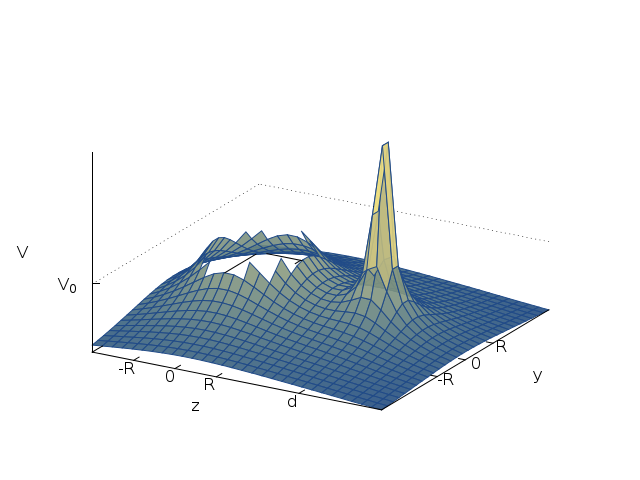
\includegraphics[scale=0.7]{V.png}
		\caption{ Potencial $V(\vec{r})$ para $\vec{r} > R$ no plano $z=0$}
	\end{figure}
	(b)
	\\
	\indent Para determinar a densidade de carga induzida podemos extrair o divergente do potencial na superficie da esfera.
	
	\[\vec{E} = - \nabla V(\vec{r}) \quad \text{e pelas condições de contorno} \quad (\vec{E_1} - \vec{E_2}) \cdot \hat{n} = \frac{\sigma}{\epsilon_0} \] 
	
	\indent Onde $\vec{E_2}$ é o campo no lado de dentro e $\vec{E_1}$ do lado de fora, o campo do lado de dentro é nulo pois trata-se de um condutor, então:
	
	\[ \sigma  = -\epsilon_0 \nabla V(\vec{r}) \cdot \hat{r} \quad \text{então} \quad \sigma  = -\epsilon_0\frac{\partial}{\partial r}V(\vec{r})\]
	
	\[\sigma = -\frac{1}{ 4 \pi } \frac{\partial }{\partial r}\Bigg[ \frac{R}{d}\frac{-q}{|\vec{r} - \frac{R^2}{d}\hat{x}|} + \frac{q}{|\vec{r} - d\hat{x}|} + \frac{4\pi \epsilon_0 R V_0}{|\vec{r}|} \Bigg]_{r=R}\]
		
	\[\sigma = -\frac{1}{ 4 \pi} \Bigg[ \frac{R}{d}\frac{q(R - \frac{R^2}{d}\hat{x}\cdot\hat{r})}{|R - \frac{R^2}{d}|^3} + \frac{q(R - d\hat{x}\cdot\hat{r})}{|R - d|^3} + \frac{4\pi \epsilon_0 V_0 }{R} \Bigg]\]
		
		
		
	\[\sigma = -\frac{1}{ 4 \pi  } \Bigg[ \frac{R}{d}\frac{q(R - \frac{R^2}{d}\sin(\theta)\cos(\phi))}{|R - \frac{R^2}{d}|^3} + \frac{q(R - d\sin(\theta)\cos(\phi))}{|R - d|^3} + \frac{4\pi \epsilon_0 V_0 }{R} \Bigg]\]
		
	\begin{figure}[h]
		\centering
		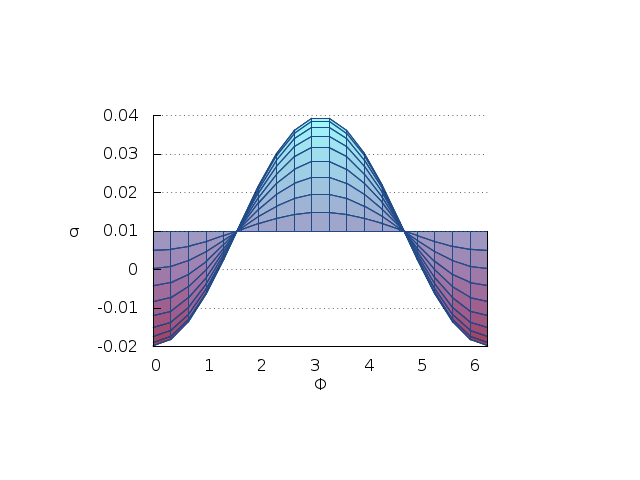
\includegraphics[scale=0.35]{Sig2.png}
		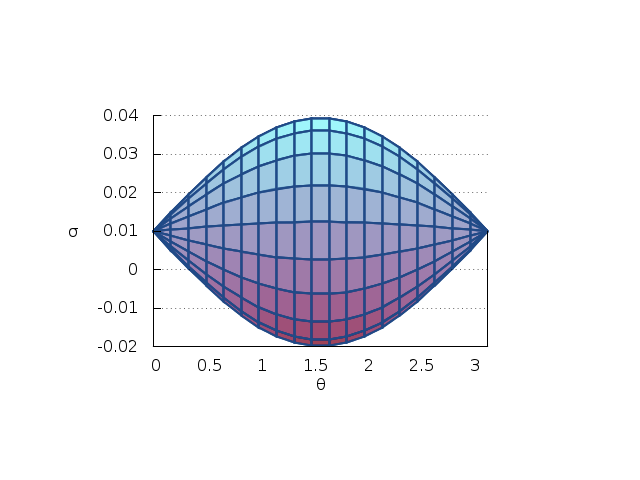
\includegraphics[scale=0.35]{Sig3.png}
		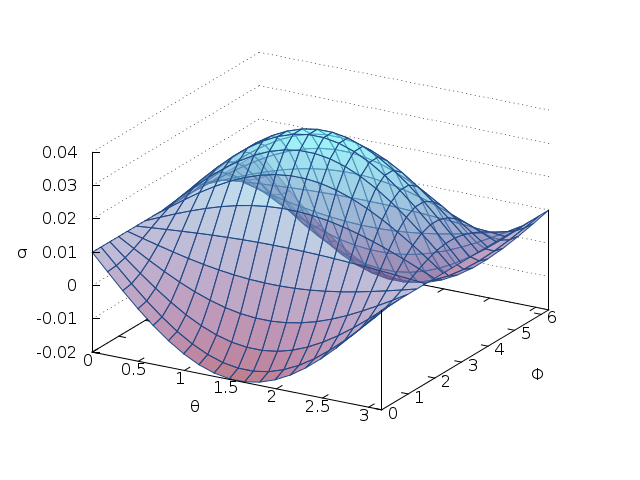
\includegraphics[scale=0.6]{Sig1.png}
		
		\caption{ $\sigma (\theta,\phi)$ na superfície da esfera adotando $\phi$ azimutal e theta polar \\ \small $0 \le \theta \le \pi$ e $0 \le \phi \le 2\pi$ }
	\end{figure}	
		\pagebreak
		(c)
		\\
		\indent Para calcular a força, voltemos ao problema imagem.
		
		\begin{center}
		\begin{tikzpicture}
		  \draw[dashed] (0,0) circle (1.5) node[above , shift={(1,1.2)}] {$V_0$};
		  \draw (-2,0) -- (10,0);
                  \draw (0,0.2) -- (0,-0.2) node[below] {$0$};
                  \draw[fill=black] (0,0) circle (0.1) node[above , shift={(0,0.2)} ] {$q_0$};
                  \draw (0.7,0.2) -- (0.7,-0.2) node[below] {$d'$};
                  \draw[fill=black] (0.7,0) circle (0.1) node[above ,shift={(0,0.2)}] {$q'$};
                  \draw (8,0.2) -- (8,-0.2) node[below] {$d$};
                  \draw[fill=black] (8,0) circle (0.1) node[above , shift={(0,0.2)} ] {$q$};
                  \draw[arrows=->] (7.8,0.1) -- (7,0.1) node[above, midway] {$\vec{F_q}$};
		\end{tikzpicture}
	\end{center}
	Temos 3 cargas agora, o que significa que teremos a contribuição de duas forças provenientes das cargas $q_0$ e $q'$ atuando sobre a carga $q$, portanto:
	
	\[ \vec{F_q} = \frac{q}{4 \pi \epsilon_0} \Bigg( \frac{q_0}{d^2} + \frac{q'}{(d-d')^2} \Bigg)\hat{x}\]
	e como já sabemos $q'$, $d'$ e $q_0$
	\[ \vec{F_q} = \frac{q}{4 \pi \epsilon_0} \Bigg( \frac{4 \pi \epsilon_0 R V_0}{d^2} - \frac{R \,q}{(d-R)^2} \Bigg)\hat{x}\]
	
\end{document}
